\subsection{Appearance editor}
\writer{Monica}

The Appearance Editor is the component which allows the user to associate a visual representation to the Petri net elements so that they can be rendered in the 3D simulation. The editor can be used by both technical and non-technical users as it only implies linking \textit{Appearance Labels} previously defined in the Geometry with predefined 3D and texture files. 

Figure \ref{fig:appearance} shows the model used by the Appearance Editor component.

\begin{figure}[htp]
\begin{center}
  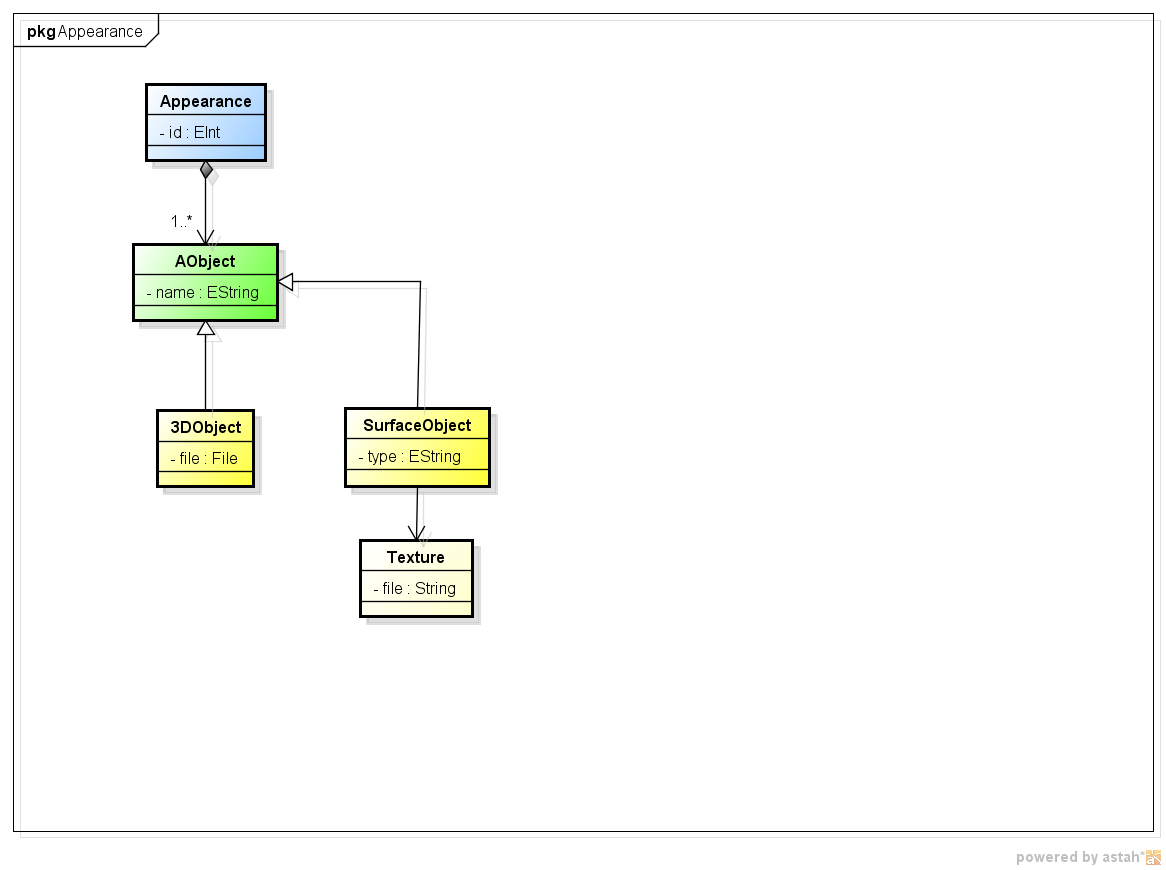
\includegraphics[width=0.8\textwidth]{image/appearance-model.png}
  \caption{Appearance Domain Model}
  \label{fig:appearance}
\end{center}
\end{figure}  

\subsubsection{Appearance Editor classes}
Next, the model will be described into more detail.

\paragraph{Appearance}
The Appearance class is simply an abstract definition of an Appearance object. Its only attribute is the \textbf{id}, of type EInt, representing an unique identifier of an Appearance object. Each Appearance object will also contain one or more AObjects.

\paragraph{AObject}
The AObject class is the class defining all the necessary information for the 3D visual representation of the Petri net. Its attributes are:
\begin{enumerate}
\item  \textbf{label}, of type EString, refers to the appearance label of a Petri net element found in its geometry  (e.g. \textit{"train"}).
\item \textbf{object3D}, of type EString, refers to the path of a 3D object file that will be used by the simulator during rendering 
\item \textbf{texture}, of type EString, referring to the path of a texture file that will be used by the simulator during rendering 
\end{enumerate}


